\section{Introduction}
\label{sec:intro}

In this note, we present estimates of CMS sensitivity to SUSY for
$5\sigma$ discovery, reach as well as 95\% C.L. limits in the mSUGRA 
framework with R-parity conservation at a proton-proton
center-of-mass of 7 TeV. This model is characterized by five 
free parameters described as follows: 

\begin{itemize}
\item $m_{0}$: the common scalar mass at the GUT scale; 
\item $m_{1/2}$: the common gaugino mass at the GUT scale; 
\item $A_{0}$: the common soft trilinear SUSY breaking parameter at
  the GUT scale; 
\item tan$\beta$: the ratio of the Higgs vacuum expectation values at
  the electroweak scale; 
\item sign $\mu$: the sign of the Higgsino mass term. 
\end{itemize}

We set $A_{0} = 0$, sign $(\mu) > 0$ and tan$\beta = 3$ in order to be
able to directly compare with recent Tevatron
results~\cite{cdf:recentSusy, d0:recentSusy}. The gluino-squark
mass plane is then scanned  via variations of $m_{0}$ and $m_{1/2}$. 
Figure~\ref{fig:tanb3_lo} shows the leading order (LO) cross sections 
as a function of $m_{0}$, $m_{1/2}$ with tan$\beta = 3$, A$_0 = 0$, $\mu > 0$.
The cross section spans over a wide range in $m_{0}-m_{1/2}$ plane, which
should be accessable during the low luminosity running period.

\vspace{3 mm}
\begin{figure}[htb]
\begin{center}
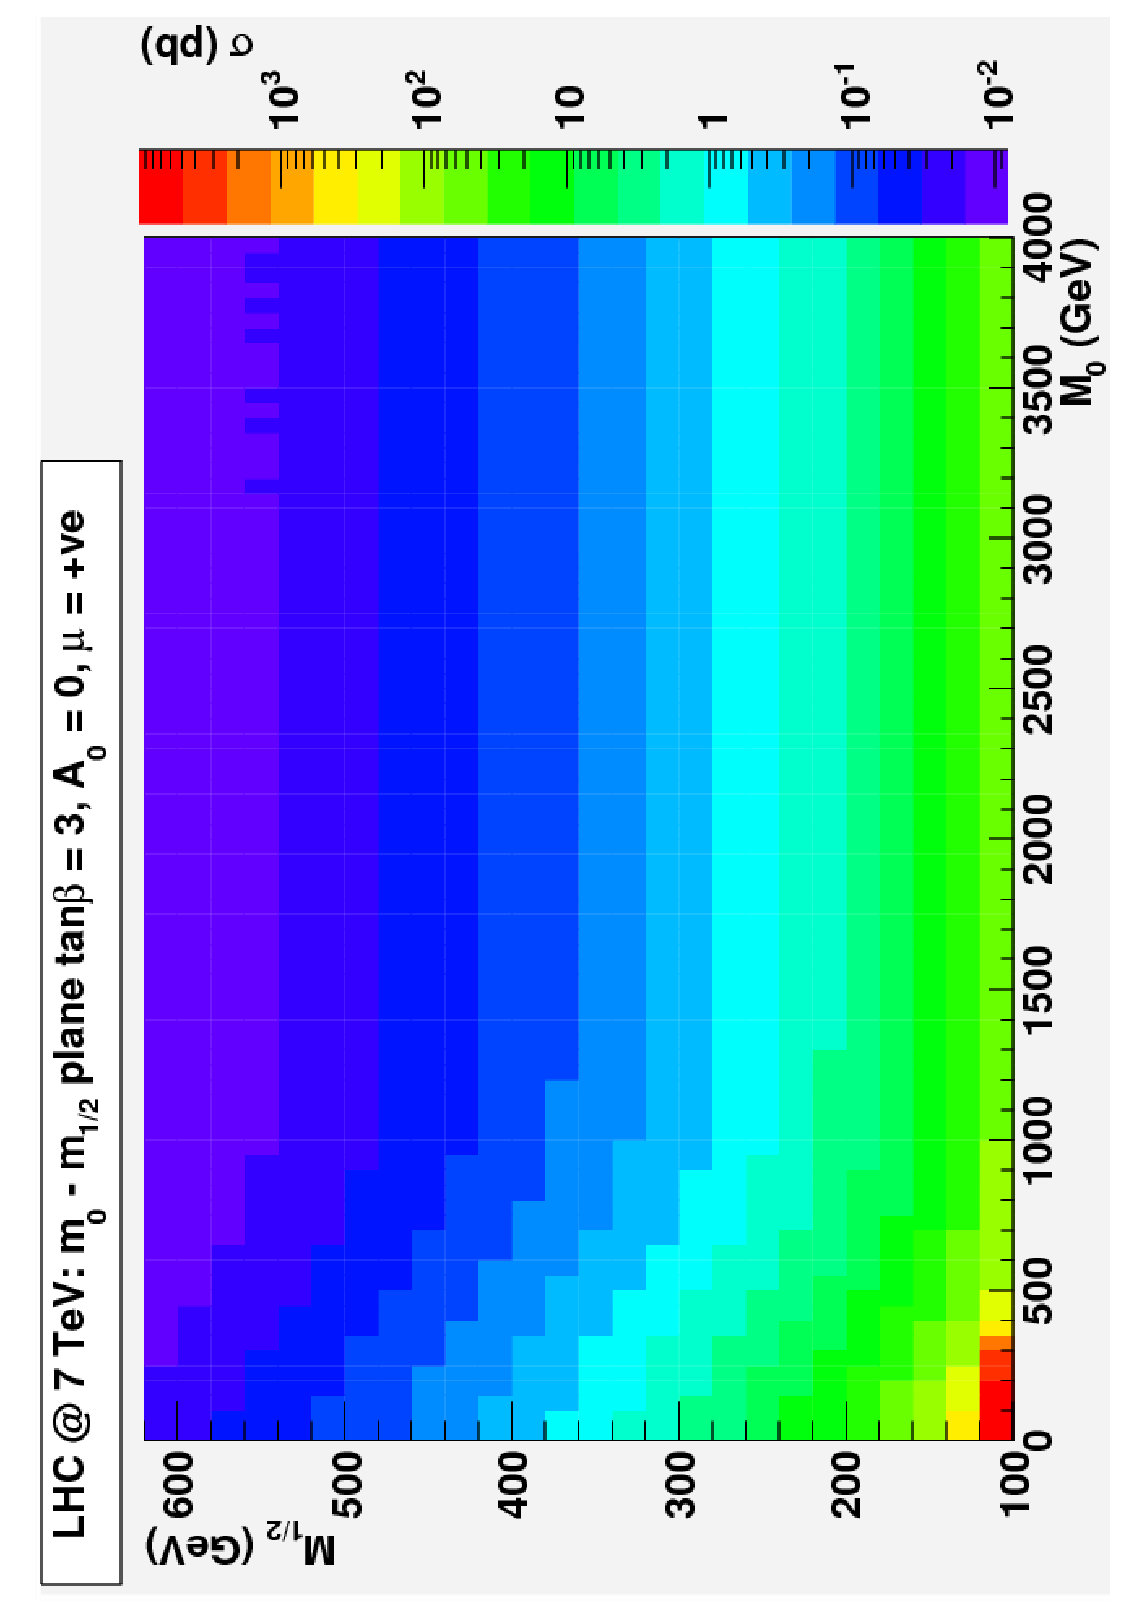
\includegraphics[angle=-90,width=0.6\linewidth]{figs/tanb3.ps}
\caption{LO cross sections as a function of $m_{0}$, $m_{1/2}$
with tan$\beta = 3$, A$_0 = 0$, $\mu > 0$. \label{fig:tanb3_lo}}
\end{center}
\end{figure}

In this framework all supersymmetric particles except the
lightest supersymmetric particle (LSP, which throughout most of the
mSUGRA parameter space is the lighest neutralino) are unstable and
thus will decay into their Standard Model (SM) counterparts right after being
produced. The cascade decay can result in di-lepton final states
associated  with several jets, plus missing transverse energy (\met~)
from the LSP.  

The note is organized as follows: in Section~\ref{sec:datasamples} we
list the Monte Carlo (MC) data samples, as well as the  software tags used
in this analysis; in Section~\ref{sec:eventselection} we describe the
same sign (SS) and opposite sign (OS) di-lepton event selection used in
this study; in Section~\ref{sec:samesign} we discuss the exclusion limits 
and mass reach using SS di-leptons followed by a similar study involving OS
di-leptons in Section~\ref{sec:osstudies}. Finally, in 
Section~\ref{sec:conclusion} we summarize the results.  

The work presented here updates previously documented studies 
in~\cite{osnote} and~\cite{ssnote} from 10 TeV center-of-mass to 7 TeV, 
and from 2 series to 3 series MC.
 
 



